\documentclass[ a4paper,
                oneside,
                toc=bibliography,
                toc=listof
                ]{scrbook}

\usepackage[ngerman]{babel} % If the thesis is in English
\usepackage {longtable}
%\usepackage[english, ngerman]{babel} % If the thesis is in German


% This class does the ISW styling for you (together with scrbook).
%
% It handles the following:
% - Proper input and font encoding (Just type, don't care about the LaTeX compiler you use or how to type German umlauts)
% - Fonts with ligatures and kerning (Tex Gyre fonts are used, part of every LaTeX installation, text is nice to read)
% - Bibliography styling for biblatex (declare your bibliography file and you are ready to go)
% - Provide command for title page (\makeISWtitle) and declaration of originality ( \declarationOfOriginality)
% - Loads packages "biblatex" and "graphics"
\usepackage[
    type=study, % master, bachelor, bachelorproject
]{iswthesis}

%Path to .bib-File(s) for BibLatex
\addbibresource{bibliography.bib}
% \addbibresource{someOtherBibFile}

\author{Lukas Schlotter}
\placeOfBirth{Stuttgart}
\major{Mechatronik}
\title{jbjhkbkj}
\titleTranslated{Wie man einen Hamster trainiert}
\matrnr{3668915}
\date{\today}
\supervisor{My supervisor, M.Sc.}
\professor{Prof. Dr.-Ing. Oliver Riedel}

\begin{document} 
    \frontmatter
    \makeISWtitle
    
    \cleardoublepage
	\setcounter{page}{1} % start at page (i) after title page
    %\declarationOfOriginality

    % Kurzfassung/Abstract
    
    \cleardoublepage
    \tableofcontents
    

    \mainmatter
    
    \chapter{Einleitung}
    Warum startet das hier mit ner 0?
    aTex allows you to manage citations within your document through the use of a separate bibtex file (filename.bib).
    
    
    \newpage
    
    Bibtex files follow a standard syntax that allow you to easily reference the citations included in that file through the use of a bibliography management package. There are multiple bibliography management packages that you can use to manage citations. \\
    This guide will demonstrate how to use biblatex which allows for the most customization.
    \section{Motivation}
    
    Dieses Bild zeigt blabla bla von dem Buch \cite{Tantau2013} und auch \cite{Kohm2013}
    
    \begin{table}[h!]
    	\centering
    	\begin{tabular}{||c c c c||} 
    		\hline
    		Col1 & Col2 & Col2 & Col3 \\ [0.5ex] 
    		\hline\hline
    		1 & 6 & 87837 & 787 \\ 
    		2 & 7 & 78 & 5415 \\
    		3 & 545 & 778 & 7507 \\
    		4 & 545 & 18744 & 7560 \\
    		5 & 88 & 788 & 6344 \\ [1ex] 
    		\hline
    	\end{tabular}
    	\caption{Table to test captions and labels.}
    	\label{table:1}
    \end{table}
	
	\section{Anforderungsdefinition}
	
	\section{Methodik}

	\chapter{Grundlagen und Stand der Technik}
	
	\section{Feldbusse}
	Feldbusse: Elektrotechnik für Maschinenbauer ab S.485\\
	\\
	Feldbusse: Profibus, CAN, Sercos
	\\
	\\	
	Ethernet basierte Feldbusse: Profinet, Ethernet/IP, EtherCAT, Sercos III \\
	Ethernetbasierte Systeme sind bereit Feldbusse abzulösen \\
	\begin{figure}[!ht]
		\centering
		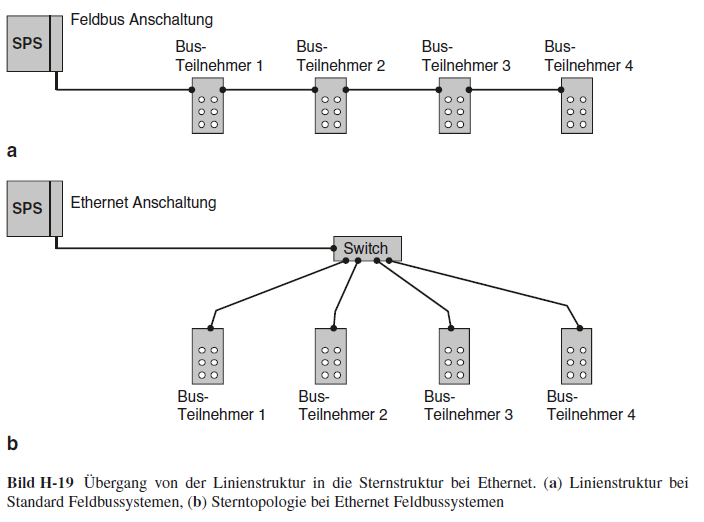
\includegraphics[width=1.0\linewidth]{./images/Feldbus vs Ethernet Anschaltung.png}
		\caption{Anschaltung Feldbus und Ethernet \cite{hering2012elektrotechnik}}
		\label{fig:Anschaltung Bus}
	\end{figure}
	\begin{figure}[!ht]
		\centering
		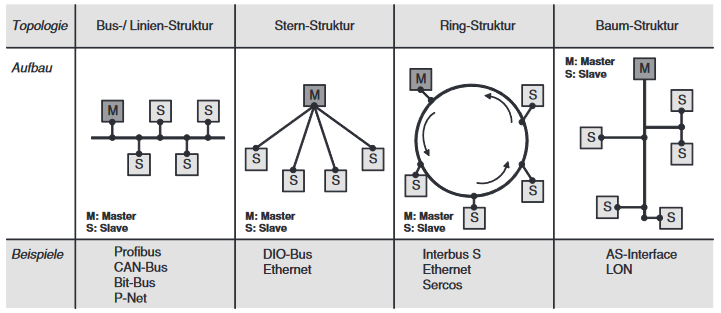
\includegraphics[width=1.0\linewidth]{./images/Topologien.png}
		\caption{Topologien}
		\label{fig:Topologien}
	\end{figure}
	Ethernet: deutlich mehr Daten als klassisch \\
	Multi-Master Bussen (z.B. CAN oder TCP/IP) vs. Mono-Master
	
	\section{TCP/IP}
	TCP/IP (Transmission Control Protocol/Internet Protocol) ist das meist verwendete Netzwerkprotokoll weltweit und zudem frei zugänglich. Durch dieses Protokoll wird definiert, wie Daten durch Netzwerkkommunikationshardware versendet und empfangen werden kann. \cite{CS9_TCP} \\
	TCP/IP ist nicht echtzeitfähig, stellt jedoch eine gute Ergänzung zu den Echtzeitprotokollen dar, um nicht zeitkritische Daten, wie z.B. zur Diagnose oder  Visualisierung zu übertragen. Bei TCP/IP handelt es sich um eine sichere Datenübertragung die Nachrichten in einen Bytestrom verpackt und entpackt. Vom Sender zum Empfänger durchlaufen die Daten vier Schichten (vgl. Abbildung \ref{fig:Schichtenmodell}). Für eine sichere fehlerfreie Übertragung werden die eigentlichen Daten ergänzt um die MAC-/IP- und TCP-Header. Das CRC-Feld stellt eine Art Prüfsumme, mit welcher die Korrektheit der übertragenen Daten überprüft wird. \cite{hering2012elektrotechnik}
	\begin{figure}[!ht]
		\centering
		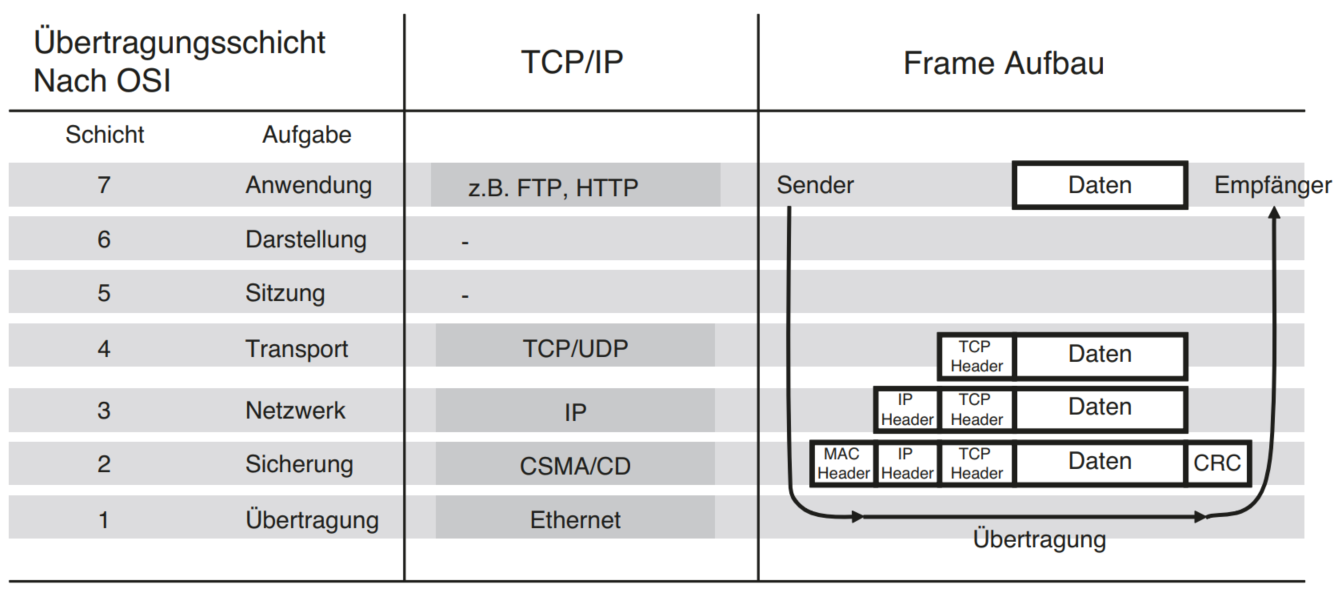
\includegraphics[width=1.0\linewidth]{./images/Schichtenmodell_TCP_IP.png}
		\caption{Schichtenmodell TCP/IP \cite{hering2012elektrotechnik}}
		\label{fig:Schichtenmodell}
	\end{figure} \\
	TCP/IP setzt sich aus den Protokollen TCP und IP zusammen.\\
	\textbf{TCP}\\
	Das Ziel von TCP ist eine fehlerfreie Datenübertragung. Hierzu muss der Empfänger die korrekt erhaltenen Daten, über eine Nachricht, die an den Sender zugesendet wird, bestätigen. Die Überprüfung der Korrektheit erfolgt mit dem CRC-Segment. Erhält dieser Sender diese Bestätigung nicht wird erneut versucht die Daten zu versenden. Hierdurch ist eine fehlerfreie und lückenlose Datenübertragung, selbst bei Netzwerkproblemen garantiert, was jedoch die Prozesse verlangsamt. Eine Alternative zu TCP ist UDP (User Datagram Protocol) . Hierbei erhält der Absender keine Bestätigung, dass die Daten korrekt empfangen wurde. Der Sender fährt direkt mit der Versendung der nächsten Pakete durch. Eine fehlerfreie Übertragung ist nicht garantiert, jedoch ist sie im Vergleich zu TCP schneller. Sowohl TCP, als auch UDP bauen auf dem Internetprotokoll IP auf. \cite{CS9_TCP}\\
	\textbf{IP} \\
	Das IP-Protokoll arbeitet auf der Internet bzw. IP-Schicht des TCP/IP-Protokolls, was der Netzwerkschicht des OSI-Modells entspricht. Es ermöglicht Datenpakete vom Sender zum Empfänger zu versenden. Hierzu werden die Daten in einzelne aufgeteilt und versendet. Eine Datenüberprüfung und Fehlerkorrektur erfolgt nicht. Dies geschieht durch das TCP-Protokoll. Das IP-Protokoll verwendet IP-Adressen, um Netzwerkknoten zu identifizieren. (https://www.vautron.de/blog/was-ist-das-internet-protokoll-ip) Es gibt zwei Versionen des IP-Protokolls IPv4 und IPv6. Bei IPv4 besteht die IP-Adresse aus 32 Bit, bei IPv6 aus 128 Bit, was die Anzahl der eindeutigen Adressen erhöht. Aufgrund der zunehmenden Geräteanzahl wird in der Zukunft IPv6 der Standard werden. Heute dominiert jedoch IPv4. Der Aufbau einer IP-Adresse nach IPv4 ist nachfolgend dargestellt. 
	
	
	
	
   	MAC-Adresse eindeutig von Gerät. Für bessere Identifiuierung aber IP-Adresse
   	\begin{figure}[!ht]
   		\centering
   		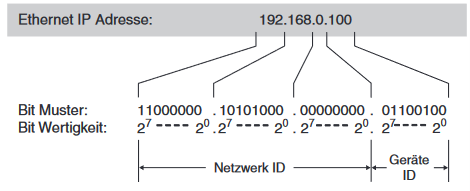
\includegraphics[width=0.70\linewidth]{./images/IP Adresse Aufbau.png}
   		\caption{Topologien}
   		\label{fig:Topologien}
   	\end{figure}
   	\\
   	Netzwerktopologien
   	
   	Bei der insbesondere ab den 80er-Jahren und auch noch heute häufig vorkommendenClient-Server-Architektur erfolgt eine Verteilung der Zuständigkeiten im Netzwerkzwischen einem sog. Client und einem sog. Server. Der Client stellt dabei Anfragen anden Server, der diese Anfragen beantwortet. Server verfügen in der Regel über deutlichmehr Rechenkapazität und mehr Speicher als Clients. Server können ihre Ressourcendurch diese hohe Rechenleistung gleichzeitig vielen Clients zur Verfügung stellen, wasdiese Architektur relativ kostengünstig macht. Mehrere Clients können üblicherweisegleichzeitig auf einen Server zugreifen, d. h. ohne sich in eine Warteschlange einreihenzu müssen. Bei einem Webrowser wie Firefox handelt es sich beispielsweise um einenClient, der wiederum auf einen Webserver zugreift. Im Kern basiert Cloud Computing aufder Client-Server-Architektur – Lösungen wie beispielsweise netzwerkbasierten Datenspeicher gab es bereits in den 80er Jahren. Im Vergleich zur Client-Server-Architekturwurden allerdings die Dienstleistungen präzisiert und nutzerorientierter gestaltet.(IT-Sicherheit)
   	Verschiedene Klassen an IP-Adressen. Meist Klasse C verwendet
   	\\
   	Weil Multi-Master-Bus braucht man CSMA/CD-Verfahren -> nicht echtzeitfähig. Lösung: Echtzeitprotokolle
   	\\
   	
   	\section{Stäubli-Roboter}
   	
   	\section{Anlagensteuerung}
   	
	\newpage
	\chapter{Konzeptionierung und Systementwurf}
	\section{Feldbus-Verbindung}
	
	\section{TCP/IP-Verbindung}
	
	\section{Datenverwertung}
	
	\begin{longtable}{|p{7cm}|p{3cm}|p{3cm}|}
		\caption{Verfügbare Daten}
		\label{table:Daten}\\
		\hline
		Daten & Zugriff & Verwendung  \\ [0.5ex] 
		\hline
		\endhead
		CPU battery test & D (CpuIO) & -  \\ 
		CPU overcurrent & D (CpuIO) & -  \\
		Fast memory state & D (CpuIO) & - \\
		CPU temperature & A (CpuIO) & Alarm, PM \\
		CPU board temperature & A (CpuIO) & Alarm, PM \\
		CPU fan speed & A (CpuIO) & Alarm, PM \\
		Free RAM & A (CpuIO) & - \\
		CFast memory remaining lifetime & A (CpuIO) & - \\
		\hline
		System management CPU usage & A (CpuUsage) & - \\
		Robot control CPU usage & A (CpuUsage) & - \\			
		Synchronous VAL 3 CPU usage & A (CpuUsage) & - \\
		Available CPU usage for VAL 3 processing& A (CpuUsage) & - \\
		User Fieldbuses CPU usage & A (CpuUsage) & - \\
		HMI CPU usage & A (CpuUsage) & - \\
		SRS connection CPU usage & A (CpuUsage) & - \\
		OPC-UA CPU usage & A (CpuUsage) & - \\
		CPU Load Score (higher is better)& A (CpuUsage) & - \\
		CPU Load Score (min) & A (CpuUsage) & - \\
		VAL 3 instructions per sequencing & A (CpuUsage) & - \\
		VAL 3 synr inst. per cyle (high priority) & A (CpuUsage) & - \\
		VAL 3 synr inst. per cyle (low priority) & A (CpuUsage) & - \\
		\hline
		Valve feedback (1.1, 1.2, 2.1, 2.2) & D (DsiIO) & - \\
		Axis brake feedback (1-6) & D (DsiIO) & - \\
		Error on valves outputs & D (DsiIO) & Alarm \\
		Error on brakes outputs & D (DsiIO) & Alarm \\
		Error on safe digital inputs & D (DsiIO) & Alarm \\
		DSI non-reduced brake supply voltage undershoot & D (DsiIO) & Alarm \\
		DSI reduced brake supply voltage undershoot & D (DsiIO) & Alarm \\
		DSI logic supply voltage undershoot & D (DsiIO) & Alarm \\
		DSI overtemperature & D (DsiIO) & Alarm \\
		\hline
		DSI board tempereature & A (DsiIO) & Alarm, PM \\
		Axis motor temperature (1-6) & A (DsiIO) & Alarm, PM \\
		Axis encoder temperature (1-6) & A (DsiIO) & Alarm, PM \\
		DSI state & A (DsiIO) & - \\
		DSI error code & A? (DsiIO) & ? Grau? Alarm \\
		Arm operation counter & A (DsiIO) & - \\
		\hline
		safe Input state (0-7) & D (DsiIoSafe) & - \\
		\hline
		Fast Input (1-2) & D (FastIO) & - \\
		Fast Output (1-2) & D (FastIO) & - \\
		\hline
		Power unit identification (bit 1-3) & D (PSIO) & - \\
		Main power state & D (PSIO) & - \\
		Internal bus voltage state & D (PSIO) & - \\
		Power unit internal temperature state & D (PSIO) & - \\
		24V state & D (PSIO) & - \\
		Buckfull mode feedback & D (PSIO) & - \\
		Memorize a power dropout & D (PSIO) & - \\
		\hline
		Brake test warning & D (Rsi9IO) & Alarm \\
		Brake test successful & D (Rsi9IO) & - \\
		Temperature of RSI board & A (Rsi9IO) & Alarm, PM \\
		Error Code of RSI board & A? (Rsi9IO) & ?Grau? Alarm \\
		\hline
		STARC board temperature & A (StarcIO) & Alarm, PM \\
		Axis drive case temperature (1-6) & A (StarcIO) & Alarm, PM \\
		Motor Winding Temperature (1-6) & A (StarcIO) & Alarm, PM \\
		Axis drive junction temperature (1-6) & A (StarcIO) & Alarm, PM \\		
		\hline
		Geschwindigkeit Endmanipulator & getSpeed(...) & - \\
		Schleppfehler Achsen 1-6 & getPositionErr()  & - \\
		Drehmoment Achsen 1-6 & getJointForce(...)  & - \\
		Bewegungsauftrag und Fortschritt & getMoveld()  & - \\
		Konfiguration des Roboters & getVersion(...)  & - \\
		Stromversorgung bei Stillstand abschalten & hibernateRobot()  & - \\
		Systemereignisse &getEvents(...)  & - \\
			
	\end{longtable}
	Durch die Verfügbarkeit von Roboterdaten ergeben sich Nutzungspotentiale, wie z.B.:
	\begin{itemize}
		\item \textbf{Überwachung und Alarm:} Bei Überschreiten von Schwellwerten oder bei Fehlermeldungen Alarm auslösen
		\item \textbf{Predictive Maintenance:} Vorhersagen treffen, wann Wartung erfolgen soll, um Ausfälle vorbeugend zu verhindern.
		\item \textbf{Datenarchivierung und Compliance:} Datenspeicherung für Schadensfall oder gesetzliche Gewährleistung
		\item \textbf{Trendanalyse:} Muster und Tendenzen in den Daten erkennen
	\end{itemize}
	
 	Prinzipiell lassen sich alle verfügbaren Daten sammeln, visualisieren und auswerten. Bei einigen dieser Daten wie z.B. des freien RAM-Speichers ist der daraus entstehende Nutzen beschränkt.	Mittels Brainstorming wurden verschiedene Anwendungsszenarien ausgedacht, im nachfolgenden sollen jedoch nur die sinnvollsten hiervon vorgestellt werden.\\
 	\textbf{Temperaturen}\\
 	Neben der Temperatur von verschiedenen Computer-Chips und Platinen, wie z.B. CPU, CPU-Platine DSI-Platine, RSI-Platine und STARC-Platine sind verschiedene Temperaturwerte von den Antrieben abrufbar. Hier sind die Temperaturen der Motoren, Encoder, Antriebsgehäuse,  Antriebswicklungen und  Steuergeräte zu nennen. Diese Daten können sowohl zur Überwachung als auch zur Predictive Maintenance verwendet werden. Bei Überschreiten eines Grenzwertes kann ein Alarm bzw. eine Warnung ausgegeben werden. Da von Seiten des Herstellers keine zulässigen Grenzwerte vorgegeben sind, müssen die aufgezeichneten Messwerte unter Berücksichtigung von Schwankungen analysiert werden und Grenzwerte festgelegt werden, ab welchen Werten das Verhalten nicht mehr als "normal" angesehen werden kann. Die Dynamik von Temperaturen ist im Allgemeinen relativ gering, da sich die Materialien aufgrund ihrer Wärmekapazität erst aufheizen müssen. Aus diesem Grund ist das Übertragen von den Temperaturwerten in vergleichsweise großen Abständen zulässig z.B. alle 15 Sekunden. Im Falle eines technischen Defektes wäre eine möglichst frühe Warnung wünschenswert, jedoch ist die Zeit bis ein Techniker den Alarm wahrnimmt und entsprechende Aktionen starten kann vergleichsweise groß, weshalb dieser Anwendungsfall kein höhere Übertragungsrate rechtfertigt. Da die Genauigkeit von vielen Temperatursensoren nur im Bereich von 0,5K liegt und sehr genaue Temperaturwerte keinen zusätzlichen Mehrwert bieten, ist eine Übertragung der Temperaturen ohne Nachkommastellen ausreichend. Dadurch lässt sich ein Temperaturwert problemlos mit einem einzelnen Byte (Werte zwischen 0 und 255°C) übertragen.\\
 	\textbf{Error-Meldungen}\\
 	Von dem Stäubli-Roboter werden einige Fehlermeldungen erfasst, wie von den Ventil und Brems-Ausgängen, den digitalen Sicherheits-Eingängen, des DSI-Chip, RSI-Chip und Bremsentests. Ebenso werden "DSI non-reduced brake supply voltage undershoot",  "DSI reduced brake supply voltage undershoot", "DSI logic supply voltage undershoot" und "DSI overtemperature" erfasst. Error-Meldungen wie diese sollen als Alarm bzw. Fehlermeldung ausgegeben werden. Ebenso ist ein Dokumentieren sinnvoll, um bei Ausfällen oder Defekten die Ursachensuche zu erleichtern. Jeder Fehler kann als Wert 1 oder 0 dargestellt werden, weshalb je Fehlermeldung ein Bit genügt. Alle Error-Meldungen lassen sich somit über 2 Bytes abbilden.\\
 	\textbf{Schleppfehler}\\
 	Der Schleppfehler entspricht der Abweichung zwischen Soll-Position und Ist-Position jeder einzelnen Achse. Ein herausstechend großer Schleppfehler kann auf Probleme mit der Steuerung, den Motoren, den Encoder oder den Achsen selbst hinweisen. Eine genaue Eingrenzung ist auf Basis der gegebenen Daten nicht möglich, jedoch ist eine Warnung sinnvoll. Zur Ermittlung der Grenze, bei deren Überschreiten eine Warnung ausgegeben werden soll, können aufgezeichnete Daten unter Berücksichtigung von Schwankungen herangezogen werden. Der Schleppfehler muss sehr regelmäßig erfasst werden, um die kontinuierliche Bewegung best möglichst abzubilden.\\
 	\textbf{Drehmoment Achsen}\\
 	Das Drehmoment der einzelnen Achsen ändert sich kontinuerlich während der Bewegung. Durch das Vergleichen der Drehmomente mit einer Referenzfahrt können  Auffälligkeiten entdeckt werden. Schleichend zunehmende Momente deuten z.B. auf fehlende Schmierung oder Lagerdefekte hin. Abrupt zunehmende Momente können durch ein Festhängen oder einen Crash verursacht werden. Eine Dokumentation der Abweichungen ist sinnvoll, um aus Gewährleistungsgründen unsachgemäße Verwendung z.B. durch einen Crash nachzuweisen. Analog zum Schleppfehler müssen auch die Drehmomente sehr kontinuierlich erfasst werden.\\
	\textbf{Sytemereignisse}\\
	Ereignisse, die auf dem Bedienpanel des Roboters dargestellt werden, lassen sich in die Schweregrade "Info", "Warning", "Error" und "Critical" unterteilen. Diese sollen beim Auftreten sofort über TCP/IP übertragen werden.
	\newpage
	\chapter{Implementierung}
	
	\section{Stäubli-Roboter in VAL3}
	
	\subsection{EtherCAT}
	
	\subsection{TCP/IP}
	Für die Implementierung der TCP/IP-Verbindung auf dem Controller des Stäubli-Roboters muss in der SRS eine Socket-Verbindung angelegt werden. Hierzu wird in der E/A-Verwaltung ein Client angelegt, welcher die IP-Adresse und den Port des Servers zugewiesen bekommt. Darüber hinaus wird ein sogenannter Timeout von 0 s gesetzt. Bei einem Timeout von 0 wird auf den Vorgang, welcher ein Lesen oder Schreiben sein kann gewartet. Bei einem Timeout kleiner 0 wird hingegen nicht bis zur Ausführung des Vorgangs gewartet. Be einem Timeout größer 0 wird hingegen eine gewisse Zeit gewährt, bis zu dieser der Timeout durchgeführt werden kann. Die Nachricht soll in diesem Fall jedoch direkt gelesen oder geschrieben werden, weshalb kein Spielraum im Rahmen des Timeouts gewährt wird. \cite{VAL3} Die Socket-Verbindung wird als E/A-Verbindung in VAL3 betrachtet, weshalb eine globale Variable mit dem Namen des Clients angelegt werden kann und hierüber auch gelesen und beschrieben werden kann. Die Socket-Verbindung wird nur dann erstellt, wenn sie ihm Rahmen des Programmablaufs z.B. durch die Befehle sioSet und sioGet benötigt wird. Der Client versucht dann eine Verbindung zum Server aufzubauen.   usepackage{ffcode}\\
	num sioGet(sio siInput, num\& nData[])\\
	Diese Funktion schreibt ein gelesenes Zeichen oder einen gelesen Array von Zeichen von siInput in das Array nData. Als Rückgabewert dient die Anzahl der gelesenen Zeichen.	
	num sioSet(sio siOutput, num\& nData[]) \\
	Mit dieser Funktion kann in VAL3 die zu übermittelnde Nachricht nData versendet werden, indem der E/A-Verbindung siOutput die Nachricht zugewiesen wird. Zurückgegeben wird die Anzahl der geschriebenen Zeichen oder "-1" im Falle des Timeouts. \\
	Das Versenden von Nachrichten erfolgt über einen Byte-Array, das heißt durch die Aneinanderreihung mehrerer Bytes. Folglich muss die zu versendete Nachricht in einen Byte-Array umgewandelt werden und beim Empfangen muss der Byte-Array interpretiert werden.\\
	num toBinary(num nValue[], num nValueSize, string sDataFormat, num\& nDataByte[])\\
	Diese Funktion wandelt einen numerischen Wert, welcher das Datenformat sDataFormat besitzt in einen Byte-Strom und speichert diesen im Array nDataByte. Über das Datenformat wird beispielsweise angegeben ob es sich um einen Gleitkommawert handelt, ob ein Vorzeichen vorliegt und ob das Little-Endian oder das Big-Endian-Format angewandt wird. Mit nDataSize kann die Anzahl der zu kodierenden Zeichen beschränkt werden.\\
	num fromBinary(num nDataByte[], num nDataSize, string sDataFormat, num\& nValue[])\\
	Umgekehrt ermöglicht diese Funktion, einen empfangen Byte-Array in numerische Werte zu konvertieren. Das Ergebnis im Datenformat nDataFormat wird in nValue gespeichert. Die Anzahl der zu decodierenden Bytes wird festgelegt durch nDataSize, wenn nicht alle Bytes des Eingangs-Array nDataByte decodiert werden sollen.
	
	\section{.NET in C\#}
	
	
	\subsection{TCP/IP}
	
   	\subsection{Datenverwertung und Visualisierung}
   	
   	\chapter{Validierung}
   	
   	\chapter{Ausblick und Fazit}
   	
   	\backmatter
   	
   	
   	\cleardoublepage
   	\listoffigures
   	\cleardoublepage
   	\listoftables
   	\cleardoublepage
   	
   	\cleardoublepage
   	\printbibliography
   	% Acronyms
   	
   	% Appendix, if needed:
   

\end{document}